% E1 through E5: results prose intentionally empty.
% This draft puts the wide placeholders on a shared page to keep their
% headings next to the visuals while the experimental prose is empty.
\FloatBarrier
\twocolumn[{%
  \begingroup
  \renewenvironment{table*}[1][]{%
    \noindent\begin{minipage}{\textwidth}\captionsetup{type=table}\centering
  }{\end{minipage}\par\vskip1pt}%
  \renewenvironment{figure*}[1][]{%
    \noindent\begin{minipage}{\textwidth}\captionsetup{type=figure}\centering
  }{\end{minipage}\par\vskip1pt}%
\subsection{End-to-End Ranking}
\label{sec:exp:e1}
% Synthetic layout preview from round2/tables-pseudocode/src/synthetic.py.
% Single full-width 27-column dual-model table with uncrowded typography & Ours row highlight.
\begin{table*}[t]
\centering
\caption{End-to-end Full ranking quality (Spearman's $\rho\uparrow$), total tokens ($\times 10^{3}\downarrow$), and isolated latency ($\text{s}\downarrow$) across six benchmarks.}
\label{tab:exp1-full}
\begingroup
\normalfont\rmfamily\fontsize{6.4}{8.3}\selectfont
\renewcommand{\qpm}[2]{\mbox{\IfBeginWith{#1}{0.}{\StrGobbleLeft{#1}{1}}{#1}\kern0.35pt{\normalfont\textcolor[HTML]{64748B}{\fontsize{4.8}{5.8}\selectfont\textpm\IfBeginWith{#2}{0.}{\StrGobbleLeft{#2}{1}}{#2}}}}}
\setlength{\tabcolsep}{0pt}
\renewcommand{\arraystretch}{0.96}
\begin{tabular*}{\textwidth}{@{\extracolsep{\fill}}l!{\hspace{2.2pt}}c!{\hspace{1.6pt}}c!{\hspace{1.6pt}}c!{\hspace{1.6pt}}c!{\hspace{1.6pt}}c!{\hspace{1.6pt}}c!{\hspace{2.6pt}}c!{\hspace{1.5pt}}c!{\hspace{1.5pt}}c!{\hspace{2.4pt}}c!{\hspace{2.4pt}}c!{\hspace{1.1pt}}c!{\hspace{1.1pt}}c!{\hspace{3.6pt}\color[HTML]{CBD5E1}\vrule width 0.55pt\hspace{3.6pt}}c!{\hspace{1.6pt}}c!{\hspace{1.6pt}}c!{\hspace{1.6pt}}c!{\hspace{1.6pt}}c!{\hspace{1.6pt}}c!{\hspace{2.6pt}}c!{\hspace{1.5pt}}c!{\hspace{1.5pt}}c!{\hspace{2.4pt}}c!{\hspace{2.4pt}}c!{\hspace{1.1pt}}c!{\hspace{1.1pt}}c@{}}
\toprule
& \multicolumn{13}{c}{\fontsize{7.2}{8.2}\selectfont\textbf{\textcolor[HTML]{1F5A8A}{Qwen3.5-9B}}} & \multicolumn{13}{c}{\fontsize{7.2}{8.2}\selectfont\textbf{\textcolor[HTML]{A63A50}{Qwen3.8-27B}}} \\
\cmidrule(lr){2-14}\cmidrule(lr){15-27}
\textbf{Method} & \multicolumn{6}{c}{Quality $\rho\uparrow$} & \multicolumn{3}{c}{Tokens ($\times 10^{3}$)$\downarrow$} & Lat.$\downarrow$ & \multicolumn{3}{c}{Rank$\downarrow$} & \multicolumn{6}{c}{Quality $\rho\uparrow$} & \multicolumn{3}{c}{Tokens ($\times 10^{3}$)$\downarrow$} & Lat.$\downarrow$ & \multicolumn{3}{c}{Rank$\downarrow$} \\
\cmidrule(lr){2-7}\cmidrule(lr){8-10}\cmidrule(lr){12-14}\cmidrule(lr){15-20}\cmidrule(lr){21-23}\cmidrule(lr){25-27}
& Q9 & DL20 & DL22 & COVID & DBP & R04 & Q9 & TREC & BEIR & s & $Q$ & $T$ & $L$ & Q9 & DL20 & DL22 & COVID & DBP & R04 & Q9 & TREC & BEIR & s & $Q$ & $T$ & $L$ \\
\midrule
Pointwise & \underline{\qpm{0.820}{0.012}} & \underline{\qpm{0.820}{0.012}} & \underline{\qpm{0.820}{0.012}} & \textbf{\qpm{0.840}{0.012}} & \textbf{\qpm{0.840}{0.012}} & \textbf{\qpm{0.840}{0.012}} & \textbf{1.00} & \textbf{2.03} & \textbf{3.12} & \textbf{1.75} & \textbf{1} & \textbf{1} & \textbf{1} & \underline{\qpm{0.840}{0.012}} & \underline{\qpm{0.840}{0.012}} & \underline{\qpm{0.840}{0.012}} & \textbf{\qpm{0.860}{0.012}} & \textbf{\qpm{0.860}{0.012}} & \textbf{\qpm{0.860}{0.012}} & \textbf{5.00} & \textbf{10.03} & \textbf{15.12} & \textbf{2.25} & \textbf{1} & \textbf{1} & \textbf{1} \\
Ext.\ Point. & \textbf{\qpm{0.840}{0.013}} & \textbf{\qpm{0.840}{0.013}} & \textbf{\qpm{0.840}{0.013}} & \underline{\qpm{0.820}{0.013}} & \underline{\qpm{0.820}{0.013}} & \qpm{0.800}{0.013} & \underline{1.10} & \underline{2.23} & \underline{3.42} & \underline{2.15} & \underline{2} & \underline{2} & \underline{2} & \textbf{\qpm{0.860}{0.013}} & \textbf{\qpm{0.860}{0.013}} & \textbf{\qpm{0.860}{0.013}} & \underline{\qpm{0.840}{0.013}} & \underline{\qpm{0.840}{0.013}} & \qpm{0.820}{0.013} & \underline{5.10} & \underline{10.23} & \underline{15.42} & \underline{2.65} & \underline{2} & \underline{2} & \underline{2} \\
Ext.\ Bubble & \qpm{0.800}{0.014} & \qpm{0.800}{0.014} & \qpm{0.800}{0.014} & \qpm{0.800}{0.014} & \qpm{0.780}{0.014} & \underline{\qpm{0.820}{0.014}} & 1.20 & 2.43 & 3.72 & 2.55 & 3 & 3 & 3 & \qpm{0.820}{0.014} & \qpm{0.820}{0.014} & \qpm{0.820}{0.014} & \qpm{0.820}{0.014} & \qpm{0.800}{0.014} & \underline{\qpm{0.840}{0.014}} & 5.20 & 10.43 & 15.72 & 3.05 & 3 & 3 & 3 \\
Ext.\ Merge & \qpm{0.780}{0.015} & \qpm{0.780}{0.015} & \qpm{0.780}{0.015} & \qpm{0.780}{0.015} & \qpm{0.800}{0.015} & \qpm{0.780}{0.015} & 1.30 & 2.63 & 4.02 & 2.95 & 4 & 4 & 4 & \qpm{0.800}{0.015} & \qpm{0.800}{0.015} & \qpm{0.800}{0.015} & \qpm{0.800}{0.015} & \qpm{0.820}{0.015} & \qpm{0.800}{0.015} & 5.30 & 10.63 & 16.02 & 3.45 & 4 & 4 & 4 \\
\midrule
ListK Sort & \qpm{0.760}{0.016} & \qpm{0.760}{0.016} & \qpm{0.760}{0.016} & \qpm{0.760}{0.016} & \qpm{0.760}{0.016} & \qpm{0.760}{0.016} & 1.40 & 3.10 & 6.00 & 3.35 & 5 & 6 & 5 & \qpm{0.780}{0.016} & \qpm{0.780}{0.016} & \qpm{0.780}{0.016} & \qpm{0.780}{0.016} & \qpm{0.780}{0.016} & \qpm{0.780}{0.016} & 5.40 & 11.10 & 18.00 & 3.85 & 5 & 6 & 5 \\
Tournament & \qpm{0.740}{0.017} & \qpm{0.740}{0.017} & \qpm{0.740}{0.017} & \qpm{0.740}{0.017} & \qpm{0.740}{0.017} & \qpm{0.740}{0.017} & 1.41 & 3.12 & 5.10 & 3.75 & 6 & 5 & 6 & \qpm{0.760}{0.017} & \qpm{0.760}{0.017} & \qpm{0.760}{0.017} & \qpm{0.760}{0.017} & \qpm{0.760}{0.017} & \qpm{0.760}{0.017} & 5.41 & 11.12 & 17.10 & 4.25 & 6 & 5 & 6 \\
\midrule
LOTUS Quick & \qpm{0.720}{0.018} & \qpm{0.720}{0.018} & \qpm{0.720}{0.018} & \qpm{0.720}{0.018} & \qpm{0.720}{0.018} & \qpm{0.720}{0.018} & 3.00 & 6.03 & 9.12 & 4.15 & 7 & 7 & 7 & \qpm{0.740}{0.018} & \qpm{0.740}{0.018} & \qpm{0.740}{0.018} & \qpm{0.740}{0.018} & \qpm{0.740}{0.018} & \qpm{0.740}{0.018} & 7.00 & 14.03 & 21.12 & 4.65 & 7 & 7 & 7 \\
\midrule
Setwise Heap & \qpm{0.700}{0.019} & \qpm{0.700}{0.019} & \qpm{0.700}{0.019} & \qpm{0.700}{0.019} & \qpm{0.700}{0.019} & \qpm{0.700}{0.019} & 3.10 & 6.23 & 9.42 & 4.55 & 8 & 8 & 8 & \qpm{0.720}{0.019} & \qpm{0.720}{0.019} & \qpm{0.720}{0.019} & \qpm{0.720}{0.019} & \qpm{0.720}{0.019} & \qpm{0.720}{0.019} & 7.10 & 14.23 & 21.42 & 5.05 & 8 & 8 & 8 \\
\midrule
\rowcolor[HTML]{EEF4FA}\textbf{SW} & \qpm{0.680}{0.020} & \qpm{0.670}{0.030} & \qpm{0.680}{0.020} & \qpm{0.680}{0.020} & \qpm{0.680}{0.020} & \qpm{0.680}{0.020} & 3.20 & 6.43 & 9.72 & 4.95 & 9 & 9 & 9 & \qpm{0.700}{0.020} & \qpm{0.690}{0.030} & \qpm{0.700}{0.020} & \qpm{0.700}{0.020} & \qpm{0.700}{0.020} & \qpm{0.700}{0.020} & 7.20 & 14.43 & 21.72 & 5.45 & 9 & 9 & 9 \\
\rowcolor[HTML]{EEF4FA}\textbf{LT($h$)} & \qpm{0.660}{0.021} & \qpm{0.670}{0.011} & \qpm{0.660}{0.021} & \qpm{0.660}{0.021} & \qpm{0.660}{0.021} & \qpm{0.660}{0.021} & 3.30 & 6.63 & 10.02 & 5.35 & 10 & 10 & 10 & \qpm{0.680}{0.021} & \qpm{0.690}{0.011} & \qpm{0.680}{0.021} & \qpm{0.680}{0.021} & \qpm{0.680}{0.021} & \qpm{0.680}{0.021} & 7.30 & 14.63 & 22.02 & 5.85 & 10 & 10 & 10 \\
\bottomrule
\end{tabular*}
\endgroup
\end{table*}

% Synthetic layout preview from round2/tables-pseudocode/src/synthetic.py.
% LIMIT omits ListK Select; places are recomputed over the displayed methods.
\begin{table*}[t]
\centering
\caption{End-to-end \LIMIT~$K{=}10$ prefix quality (nDCG@10), total tokens ($\times 10^{3}$), and isolated latency across six benchmarks.}
\label{tab:exp1-limit}
\begingroup
\normalfont\rmfamily\fontsize{6.5}{8.2}\selectfont
\renewcommand{\qpm}[2]{\mbox{\IfBeginWith{#1}{0.}{\StrGobbleLeft{#1}{1}}{#1}{\fontsize{5.3}{6.5}\selectfont\textpm\IfBeginWith{#2}{0.}{\StrGobbleLeft{#2}{1}}{#2}}}}
\setlength{\tabcolsep}{0.15pt}
\renewcommand{\arraystretch}{0.90}
\begin{tabular*}{\textwidth}{@{\extracolsep{\fill}}l!{\hspace{1.35pt}}c!{\hspace{0.35pt}}c!{\hspace{0.35pt}}c!{\hspace{0.35pt}}c!{\hspace{0.35pt}}c!{\hspace{0.35pt}}c!{\hspace{1.35pt}}c!{\hspace{0.35pt}}c!{\hspace{0.35pt}}c!{\hspace{1.35pt}}c!{\hspace{1.35pt}}c!{\hspace{0.35pt}}c!{\hspace{0.35pt}}c!{\hspace{2.5pt}}c!{\hspace{0.35pt}}c!{\hspace{0.35pt}}c!{\hspace{0.35pt}}c!{\hspace{0.35pt}}c!{\hspace{0.35pt}}c!{\hspace{1.35pt}}c!{\hspace{0.35pt}}c!{\hspace{0.35pt}}c!{\hspace{1.35pt}}c!{\hspace{1.35pt}}c!{\hspace{0.35pt}}c!{\hspace{0.35pt}}c@{}}
\toprule
& \multicolumn{13}{c}{\fontsize{7}{8}\selectfont\textbf{Qwen3.5-9B}} & \multicolumn{13}{c}{\fontsize{7}{8}\selectfont\textbf{Qwen3.8-27B}} \\
\cmidrule(lr){2-14}\cmidrule(lr){15-27}
Method & \multicolumn{6}{c}{nDCG@10} & \multicolumn{3}{c}{Tokens $\times 10^{3}$} & Lat. & \multicolumn{3}{c}{Rank} & \multicolumn{6}{c}{nDCG@10} & \multicolumn{3}{c}{Tokens $\times 10^{3}$} & Lat. & \multicolumn{3}{c}{Rank} \\
\cmidrule(lr){2-7}\cmidrule(lr){8-10}\cmidrule(lr){12-14}\cmidrule(lr){15-20}\cmidrule(lr){21-23}\cmidrule(lr){25-27}
& Q9 & DL20 & DL22 & COVID & DBP & R04 & Q9 & TREC & BEIR & s & $Q$ & $T$ & $L$ & Q9 & DL20 & DL22 & COVID & DBP & R04 & Q9 & TREC & BEIR & s & $Q$ & $T$ & $L$ \\
\midrule
Pointwise & \underline{\qpm{0.780}{0.012}} & \underline{\qpm{0.780}{0.012}} & \underline{\qpm{0.780}{0.012}} & \textbf{\qpm{0.800}{0.012}} & \textbf{\qpm{0.800}{0.012}} & \textbf{\qpm{0.800}{0.012}} & \textbf{1.70} & \textbf{3.43} & \textbf{5.22} & \textbf{2.05} & \textbf{1} & \textbf{1} & \textbf{1} & \underline{\qpm{0.800}{0.012}} & \underline{\qpm{0.800}{0.012}} & \underline{\qpm{0.800}{0.012}} & \textbf{\qpm{0.820}{0.012}} & \textbf{\qpm{0.820}{0.012}} & \textbf{\qpm{0.820}{0.012}} & \textbf{5.70} & \textbf{11.43} & \textbf{17.22} & \textbf{2.55} & \textbf{1} & \textbf{1} & \textbf{1} \\
Ext. Pointwise & \textbf{\qpm{0.800}{0.013}} & \textbf{\qpm{0.800}{0.013}} & \textbf{\qpm{0.800}{0.013}} & \underline{\qpm{0.780}{0.013}} & \underline{\qpm{0.780}{0.013}} & \qpm{0.760}{0.013} & \underline{1.80} & \underline{3.63} & \underline{5.52} & \underline{2.45} & \underline{2} & \underline{2} & \underline{2} & \textbf{\qpm{0.820}{0.013}} & \textbf{\qpm{0.820}{0.013}} & \textbf{\qpm{0.820}{0.013}} & \underline{\qpm{0.800}{0.013}} & \underline{\qpm{0.800}{0.013}} & \qpm{0.780}{0.013} & \underline{5.80} & \underline{11.63} & \underline{17.52} & \underline{2.95} & \underline{2} & \underline{2} & \underline{2} \\
Ext. Bubble & \qpm{0.760}{0.014} & \qpm{0.760}{0.014} & \qpm{0.760}{0.014} & \qpm{0.760}{0.014} & \qpm{0.740}{0.014} & \underline{\qpm{0.780}{0.014}} & 1.90 & 3.83 & 5.82 & 2.85 & 3 & 3 & 3 & \qpm{0.780}{0.014} & \qpm{0.780}{0.014} & \qpm{0.780}{0.014} & \qpm{0.780}{0.014} & \qpm{0.760}{0.014} & \underline{\qpm{0.800}{0.014}} & 5.90 & 11.83 & 17.82 & 3.35 & 3 & 3 & 3 \\
Ext. Merge & \qpm{0.740}{0.015} & \qpm{0.740}{0.015} & \qpm{0.740}{0.015} & \qpm{0.740}{0.015} & \qpm{0.760}{0.015} & \qpm{0.740}{0.015} & 2.00 & 4.03 & 6.12 & 3.25 & 4 & 4 & 4 & \qpm{0.760}{0.015} & \qpm{0.760}{0.015} & \qpm{0.760}{0.015} & \qpm{0.760}{0.015} & \qpm{0.780}{0.015} & \qpm{0.760}{0.015} & 6.00 & 12.03 & 18.12 & 3.75 & 4 & 4 & 4 \\
\midrule
Tournament & \qpm{0.700}{0.017} & \qpm{0.700}{0.017} & \qpm{0.700}{0.017} & \qpm{0.700}{0.017} & \qpm{0.700}{0.017} & \qpm{0.700}{0.017} & 2.11 & 4.52 & 7.20 & 4.05 & 5 & 5 & 5 & \qpm{0.720}{0.017} & \qpm{0.720}{0.017} & \qpm{0.720}{0.017} & \qpm{0.720}{0.017} & \qpm{0.720}{0.017} & \qpm{0.720}{0.017} & 6.11 & 12.52 & 19.20 & 4.55 & 5 & 5 & 5 \\
\midrule
Lotus Quick & \qpm{0.680}{0.018} & \qpm{0.680}{0.018} & \qpm{0.680}{0.018} & \qpm{0.680}{0.018} & \qpm{0.680}{0.018} & \qpm{0.680}{0.018} & 3.70 & 7.43 & 11.22 & 4.45 & 6 & 6 & 6 & \qpm{0.700}{0.018} & \qpm{0.700}{0.018} & \qpm{0.700}{0.018} & \qpm{0.700}{0.018} & \qpm{0.700}{0.018} & \qpm{0.700}{0.018} & 7.70 & 15.43 & 23.22 & 4.95 & 6 & 6 & 6 \\
\midrule
Setwise Heap & \qpm{0.660}{0.019} & \qpm{0.660}{0.019} & \qpm{0.660}{0.019} & \qpm{0.660}{0.019} & \qpm{0.660}{0.019} & \qpm{0.660}{0.019} & 3.80 & 7.63 & 11.52 & 4.85 & 7 & 7 & 7 & \qpm{0.680}{0.019} & \qpm{0.680}{0.019} & \qpm{0.680}{0.019} & \qpm{0.680}{0.019} & \qpm{0.680}{0.019} & \qpm{0.680}{0.019} & 7.80 & 15.63 & 23.52 & 5.35 & 7 & 7 & 7 \\
\midrule
SW & \qpm{0.640}{0.020} & \qpm{0.630}{0.030} & \qpm{0.640}{0.020} & \qpm{0.640}{0.020} & \qpm{0.640}{0.020} & \qpm{0.640}{0.020} & 3.90 & 7.83 & 11.82 & 5.25 & 8 & 8 & 8 & \qpm{0.660}{0.020} & \qpm{0.650}{0.030} & \qpm{0.660}{0.020} & \qpm{0.660}{0.020} & \qpm{0.660}{0.020} & \qpm{0.660}{0.020} & 7.90 & 15.83 & 23.82 & 5.75 & 8 & 8 & 8 \\
LT($h$) & \qpm{0.620}{0.021} & \qpm{0.630}{0.011} & \qpm{0.620}{0.021} & \qpm{0.620}{0.021} & \qpm{0.620}{0.021} & \qpm{0.620}{0.021} & 4.00 & 8.03 & 12.12 & 5.65 & 9 & 9 & 9 & \qpm{0.640}{0.021} & \qpm{0.650}{0.011} & \qpm{0.640}{0.021} & \qpm{0.640}{0.021} & \qpm{0.640}{0.021} & \qpm{0.640}{0.021} & 8.00 & 16.03 & 24.12 & 6.15 & 9 & 9 & 9 \\
\bottomrule
\end{tabular*}
\endgroup
\end{table*}


\subsection{Cost Model}
\label{sec:exp:e2}
{\graphicspath{{fig/e2/out/}}%
% E2. Twelve independent PDFs + single-row shared legend. Full width: 504.4bp.
% Six at 83.15bp leave room for regular flexible gutters; no negative overlap.
\newcommand{\eTwoDiamond}{\makebox[3.48bp][c]{\raisebox{0.2bp}{
\includegraphics[width=4.2bp]{e2-role-diamond.pdf}}}}
% Anchor the annotations on the upper-right pane of the projected 3-D box.
% Distances are in the unchanged 83.15 bp panel, measured from top/right.
\newsavebox{\eTwoPanelGraphic}
\newcommand{\eTwoInteriorRow}[2]{%
  \makebox[0pt][r]{%
    \raisebox{\dimexpr\ht\eTwoPanelGraphic-#1\relax}[0pt][0pt]{%
      \fontsize{6.2bp}{7bp}\selectfont\makebox[22.3bp][l]{#2}}%
    \kern19.96bp}}
\newcommand{\eTwoAnnotated}[3]{%
  \begin{minipage}{83.15bp}\centering
    \sbox{\eTwoPanelGraphic}{\includegraphics[width=\linewidth,trim=4.05bp 2.2bp 1.35bp 3.2bp,clip]{#1}}%
    \usebox{\eTwoPanelGraphic}%
    \eTwoInteriorRow{26.89bp}{#2}%
    \eTwoInteriorRow{33.77bp}{#3}%
  \end{minipage}}

\begin{figure*}[t]
\centering
\setlength{\subfigtopskip}{1pt}\setlength{\subfigcapskip}{1pt}\setlength{\subfigbottomskip}{1pt}

\includegraphics[width=325bp]{e2-legend.pdf}\par
\subfigure[Syn-A, LT, Full]{\eTwoAnnotated{panels/p01.pdf}{\textcolor[HTML]{087F9B}{\ding{72}} (13,1)}{\textcolor[HTML]{DA821E}{\eTwoDiamond} (22,1)}}\hfill%
\subfigure[Syn-B, LT, Full]{\eTwoAnnotated{panels/p02.pdf}{\textcolor[HTML]{087F9B}{\ding{72}} (15,1)}{\textcolor[HTML]{DA821E}{\eTwoDiamond} (6,1)}}\hfill%
\subfigure[Syn-C, LT, Full]{\eTwoAnnotated{panels/p03.pdf}{\textcolor[HTML]{087F9B}{\ding{72}}\kern0.9bp\textcolor[HTML]{DA821E}{\eTwoDiamond} (8,1)}{}}\hfill%
\subfigure[Syn-D, LT, \textsf{LIMIT}~10]{\eTwoAnnotated{panels/p04.pdf}{\textcolor[HTML]{087F9B}{\ding{72}} (12,1)}{\textcolor[HTML]{DA821E}{\eTwoDiamond} (2,10)}}\hfill%
\subfigure[Syn-E, LT, \textsf{LIMIT}~10]{\eTwoAnnotated{panels/p05.pdf}{\textcolor[HTML]{087F9B}{\ding{72}} (7,1)}{\textcolor[HTML]{DA821E}{\eTwoDiamond} (13,1)}}\hfill%
\subfigure[Syn-F, LT, \textsf{LIMIT}~10]{\eTwoAnnotated{panels/p06.pdf}{\textcolor[HTML]{087F9B}{\ding{72}} (19,1)}{\textcolor[HTML]{DA821E}{\eTwoDiamond} (14,2)}}\par
\vspace{4.5bp}
\subfigure[Syn-G, SW, Full]{\eTwoAnnotated{panels/p07.pdf}{\textcolor[HTML]{087F9B}{\ding{72}} (6,1)}{\textcolor[HTML]{DA821E}{\eTwoDiamond} (11,1)}}\hfill%
\subfigure[Syn-H, SW, Full]{\eTwoAnnotated{panels/p08.pdf}{\textcolor[HTML]{087F9B}{\ding{72}} (11,1)}{\textcolor[HTML]{DA821E}{\eTwoDiamond} (6,2)}}\hfill%
\subfigure[Syn-I, SW, Full]{\eTwoAnnotated{panels/p09.pdf}{\textcolor[HTML]{087F9B}{\ding{72}}\kern0.9bp\textcolor[HTML]{DA821E}{\eTwoDiamond} (9,1)}{}}\hfill%
\subfigure[Syn-J, SW, \textsf{LIMIT}~10]{\eTwoAnnotated{panels/p10.pdf}{\textcolor[HTML]{087F9B}{\ding{72}} (9,1)}{\textcolor[HTML]{DA821E}{\eTwoDiamond} (2,10)}}\hfill%
\subfigure[Syn-K, SW, \textsf{LIMIT}~10]{\eTwoAnnotated{panels/p11.pdf}{\textcolor[HTML]{087F9B}{\ding{72}} (12,1)}{\textcolor[HTML]{DA821E}{\eTwoDiamond} (20,1)}}\hfill%
\subfigure[Syn-L, SW, \textsf{LIMIT}~10]{\eTwoAnnotated{panels/p12.pdf}{\textcolor[HTML]{087F9B}{\ding{72}} (18,1)}{\textcolor[HTML]{DA821E}{\eTwoDiamond} (14,1)}}\par
\caption{Front axis $k$ (fan-in), depth axis $h$ (SW per-run quota; LT segment length); vertical merge input tokens $\times 10^{3}$. Vertical ranges adapt per panel; compare numeric ticks, not apparent heights across panels. Stars mark illustrative minima over shown configurations; hollow diamonds mark model-selected configurations at the illustrative reference cost.}
\label{fig:e2-surface-exp5-12}
\end{figure*}
}

  \endgroup
  \par\vspace{0pt}%
}]
\begingroup
\placeexperimentfigures
\Needspace{105pt}
\subsection{Large-Scale Ranking}
\label{sec:exp:scale}
{\graphicspath{{fig/experiments/figures/e3-one-row/}}%
% E3: selected 1x4 overlay, with native subfigure captions and vector panels.
\begin{figure}[t]
\setlength{\subfigcapskip}{1pt}\setlength{\subfigtopskip}{0pt}\setlength{\subfigbottomskip}{1pt}
\centering

\includegraphics[width=\columnwidth]{config-legend.pdf}\par

\includegraphics[width=\columnwidth]{kind-legend.pdf}\par
\subfigure[SW, Full]{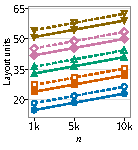
\includegraphics[width=.274716\columnwidth]{overlay-sw-full.pdf}}%
\subfigure[SW, LIMIT]{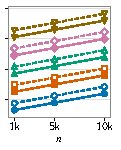
\includegraphics[width=.241761333\columnwidth]{overlay-sw-limit10.pdf}}%
\subfigure[LT, Full]{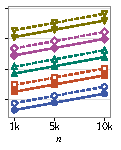
\includegraphics[width=.241761333\columnwidth]{overlay-lt-full.pdf}}%
\subfigure[LT, LIMIT]{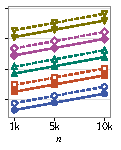
\includegraphics[width=.241761333\columnwidth]{overlay-lt-limit10.pdf}}
\caption{Scale scaffold. Predicted (dashed, hollow) and Reference (solid, filled) share each panel. Colors and marker shapes retain fixed $(k,h)$ configurations; SW first five, LT last five. Shared axes: linear input size $n$ and synthetic layout units, not tokens or time. Full and LIMIT reuse fixture curves; offsets are not prediction error.}
\label{fig:e3-scale}
\end{figure}
}

\Needspace{440pt}
\subsection{Prefix Cache}
\label{sec:exp:cache}
{\graphicspath{{fig/experiments/figures/e4a-c2/}}%
% Eight real subfigures, local spacing only. All panel assets/data unchanged.
\begin{figure}[t]
\centering
\begingroup
\setlength{\subfigcapskip}{1pt}
\setlength{\subfigtopskip}{0pt}
\setlength{\subfigbottomskip}{0pt}
\renewcommand{\subcapsize}{\fontsize{6.4}{7.4}\selectfont}

\includegraphics[width=\columnwidth]{joined-legend.pdf}\par\vspace{2pt}
{\fontsize{6}{7}\selectfont In each panel: DL20 (left)\quad\textbar\quad COVID (right)}\par\vspace{1pt}
\begin{minipage}{\columnwidth}\centering
\newlength{\eFourPanelWidth}
\setlength{\eFourPanelWidth}{0.4912\linewidth}
% Explicit fixed caption box avoids class/font interactions with subfigure's temp dimensions.
\makeatletter
\renewcommand{\@makesubfigurecaption}[2]{\hbox to\eFourPanelWidth{\hfil{\fontsize{6.4}{7.4}\selectfont #1#2}\hfil}}
\makeatother
% Trim only verified empty PDF bottom margins: 0.5bp (rows1--3), 6bp (row4).
\newcommand{\eFourPanel}[2]{\begin{minipage}{\eFourPanelWidth}\centering\offinterlineskip
\hbox{\includegraphics[width=\linewidth,trim=0bp #2 0bp 0bp,clip]{#1}}\kern1bp
\hbox to\linewidth{\hspace*{0.1610\linewidth}\hfil{\fontsize{6.2}{7.2}\selectfont $(k,h)$}\hfil}\kern0bp
\end{minipage}}
\subfigure[SW Full, n = 100]{\eFourPanel{n100-r1.pdf}{0.5bp}}%
\hfill
\subfigure[SW Full, n = 500]{\eFourPanel{n500-r1.pdf}{0.5bp}}\par\vspace{1pt}
\subfigure[SW LIMIT 10, n = 100]{\eFourPanel{n100-r2.pdf}{0.5bp}}%
\hfill
\subfigure[SW LIMIT 10, n = 500]{\eFourPanel{n500-r2.pdf}{0.5bp}}\par\vspace{1pt}
\subfigure[LT Full, n = 100]{\eFourPanel{n100-r3.pdf}{0.5bp}}%
\hfill
\subfigure[LT Full, n = 500]{\eFourPanel{n500-r3.pdf}{0.5bp}}\par\vspace{1pt}
\subfigure[LT LIMIT 10, n = 100]{\eFourPanel{n100-r4.pdf}{6bp}}%
\hfill
\subfigure[LT LIMIT 10, n = 500]{\eFourPanel{n500-r4.pdf}{6bp}}\par\vspace{1pt}
\end{minipage}\par\vspace{1pt}

\endgroup
\caption{Layout placeholder. Prefix-cache sensitivity ($\beta=0$, $m=20$). $U$ is total logical input including cache hits $Q$; $\beta$ weights hits relative to non-hits. Columns distinguish $n$; rows distinguish family/mode. Horizontal axes show $(k,h)$ within each dataset segment. Each panel concatenates DL20 (left) and TREC-COVID (right, abbreviated COVID in the shared key) as independent categories; no curve crosses the divider. Off shows $U_{\mathrm{off}}$; On-cold shows $U_{\mathrm{on}}-Q_{\mathrm{on}}$ from separate executions. Stars mark displayed minima; diamonds mark model-selected configurations at their displayed cost. Ranges are shared within $n$, not between $n$. Minima are over displayed configurations only.}
\label{fig:e4a-c2}
\end{figure}
}
{\graphicspath{{fig/experiments/figures/e4b/}}%
% Standalone single-column vector trial from the existing synthetic fixture.
\begin{figure}[t]
  \centering
  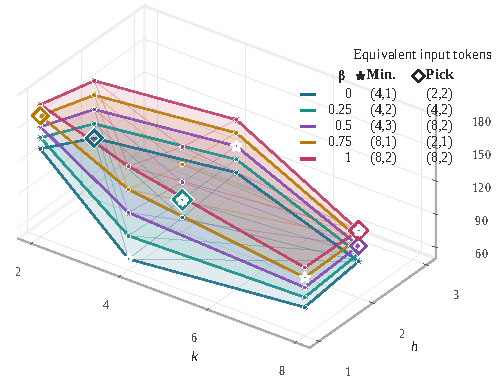
\includegraphics[width=\columnwidth]{fig/experiments/fig09-cache-discount/fig09-cache-discount-sensitivity.pdf}
  \caption{On-cold equivalent cost $C_\beta$ across five cache factors $\beta$. Stars mark empirical minima; diamonds mark planner picks.}
  \label{fig:e4b-beta}
\end{figure}
}
{\graphicspath{{fig/experiments/figures/e4c/}}%
% E4c. Single-column 2 by 2, included by integration/main.tex.
% Graphic path: figures/e4c/
\begin{figure}[t]
  \centering
  {\setlength{\subfigcapskip}{1pt}\setlength{\subfigtopskip}{0pt}\setlength{\subfigbottomskip}{0pt}
  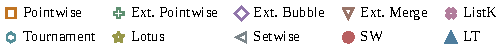
\includegraphics[width=0.87828\columnwidth]{e4c-legend.pdf}\\[-1pt]
  \subfigure[Full, Off]{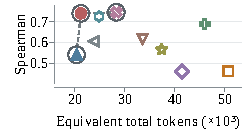
\includegraphics[width=.49\columnwidth]{panels/e4c-full-off.pdf}}\hfill
  \subfigure[Full, On-cold]{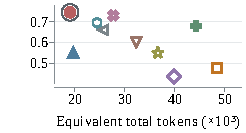
\includegraphics[width=.49\columnwidth]{panels/e4c-full-on-cold.pdf}}\\[-2pt]
  \subfigure[LIMIT 10, Off]{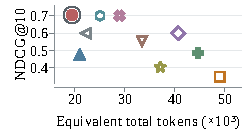
\includegraphics[width=.49\columnwidth]{panels/e4c-topk-off.pdf}}\hfill
  \subfigure[LIMIT 10, On-cold]{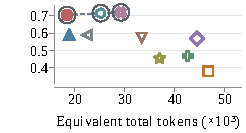
\includegraphics[width=.49\columnwidth]{panels/e4c-topk-on-cold.pdf}}}

  \caption{Layout placeholder. Method means weight DL20 and COVID equally. On denotes On-cold.
  Cost is $U+O$ (Off) or $U-Q+O$ (On, $\beta=0$), with output tokens $O$, not currency.
  Filled marks highlight SW/LT; rings mark non-dominated means.
  Dashed links imply no fit, extrapolation, or significance.}
  \label{fig:e4c-quality-cost}
\end{figure}
}

\Needspace{160pt}
\subsection{Varying the Limit and Full Ranking}
\label{sec:exp:limit-sweep}
% Cost only: four independently rendered panels in a single-column 2x2 group; quality assets retained.
\begin{figure}[t]
\centering
\setlength{\subfigcapskip}{-1pt}\setlength{\subfigtopskip}{0pt}\setlength{\subfigbottomskip}{0pt}

\includegraphics[width=\columnwidth]{fig/experiments/fig10-limit-sweep/fig10-requested-k-cost-legend.pdf}\par
\vspace{1pt}
\subfigure[\fontsize{6.3bp}{7bp}\selectfont DL20, Off]{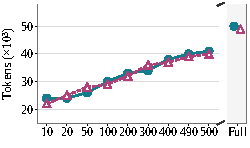
\includegraphics[width=.5\columnwidth]{fig/experiments/fig10-limit-sweep/fig10-requested-k-cost-a-dl20-off.pdf}}%
\subfigure[\fontsize{6.3bp}{7bp}\selectfont DL20, On-cold]{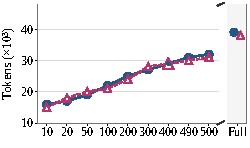
\includegraphics[width=.5\columnwidth]{fig/experiments/fig10-limit-sweep/fig10-requested-k-cost-b-dl20-on-cold.pdf}}\par\vspace{1pt}
\subfigure[\fontsize{6.3bp}{7bp}\selectfont COVID, Off]{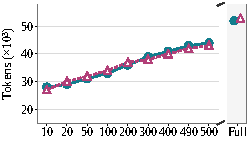
\includegraphics[width=.5\columnwidth]{fig/experiments/fig10-limit-sweep/fig10-requested-k-cost-c-covid-off.pdf}}%
\subfigure[\fontsize{6.3bp}{7bp}\selectfont COVID, On-cold]{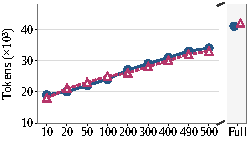
\includegraphics[width=.5\columnwidth]{fig/experiments/fig10-limit-sweep/fig10-requested-k-cost-d-covid-on-cold.pdf}}\par
{\fontsize{6.3bp}{7bp}\selectfont Requested $K$ (categorical); Full is separate}\par
\caption{Equivalent input-token cost across requested \LIMIT~$K$ prefixes and materialized Full ranking under cache Off and On-cold ($\beta{=}0$).}
\label{fig:e5-limit-sweep}
\end{figure}

\endgroup
